\chapter{Outlier Detection}

An \textbf{outlier} (anomaly) is an observation that doesn't fit the distribution of the data for normal instances, i.e., is unlikely under the distribution of the majority of instances. Outlier (anomaly) detection has the goal of finding these anomalies in datasets. Although outliers are by definition unusual, their discovery and analysis may provide critical insights on the data, in applications like fraud detection, intruder detection, ecosystem disturbances, medicine and public health, aviation safety, and so on. In all these fields, finding exceptional events or objects is often the main focus of analysis: in fraud detection we're interested in finding anomalous credit card transactions; in intrusion detection attacks can be identified by noticing weird behaviour in systems and networks.

Outliers can be caused by natural variation in values or data belonging to a minority class, or may be caused by errors. In comparison, \textbf{noise} is a random error addition to data typically caused by imprecision during measurements; it does not necessarily produce unusual values or objects, and is normally not interesting per se. Also, data objects may be outliers only for some attributes, or considering all of them. Identifying outliers in a multivariate setting can be challenging, especially when the dimensionality is high.

There are two ways in which an outlier detection method can be used. In the first one, given a dataset with both normal and anomalous instances, we are required to identify these anomalies. In the second one, we're also provided a test set of instances which we want to classify as either outliers or normal data objects. All the techniques presented in the next section can operate in the first way, and most of them (with a few exceptions) can operate in the second way.

\section{Characteristics of Outlier Detection Methods}

\begin{itemize}
    \item \textbf{Model-based vs. Model-free}: many approaches build actual models that can be used to identify whether a test instance is anomalous or not. Most \textbf{model-based} techniques construct a model trained on the normal class and identify any data point that does not fit the model. Alternatively, a model can be trained on both normal and anomalous data, and outliers are identified as those data points which are more likely to belong to the anomalous class. Both cases don't necessarily need label data (i.e., models can be trained in an unsupervised way), since they can make assumptions about the nature of the anomalous class.

    On the other hand, \textbf{model-free} approaches don't explicitly construct a model that characterizes the distribution of the anomalous and/or normal class. Instead, they directly identify instances as outliers without the need for any training, using a simpler calculation.

    If the ground truth of anomalies is available, we could define a classification problem to find outliers and solve it using popular machine learning models (ensemble models, support vector machines, deep neural networks,...). The dataset would often be unbalanced, so ad-hoc formulations should be adopted.

    \item \textbf{Global vs. Local}: some approaches consider the global context, building a model or computing an output considering the entire dataset, or by only considering the local context of each data instance; specifically, an outlier detection approach is local if its output on a given instance does not change if instances outside the local neighborhood of that point are modified or removed.

    Some approaches may be both, either because the reference set for an instance varies automatically during execution, or because it can be set by an hyperparameter.

    \item \textbf{Label vs. Score}: different approaches produce outputs in different formats. Some produce a binary \textbf{anomaly label}, and each object is identified as either an outlier or a normal instance. Others produce an \textbf{anomaly score}, indicating how strongly an instance is likely to be an anomaly. After calculating the score of a set of instances, a ranking can be obtained to identify the top-most scoring anomalies. Optionally, a cut-off threshold can be set so that all instances with a score above that are definitely classified as outliers, while the ones below are normal instances.
\end{itemize}
A very simple visual technique to find outliers is using boxplots and scatterplots. However, they do not return explicit values, and are highly subjective, since they cannot find points that are outliers when considering all dimensions. An alternative is calculating the \textbf{Histogram-based Outlier Score}, which is done by building histograms for each feature. These histograms are then normalized to the $[0,1]$ range, and the \textbf{HBOS} for each record $p$ is computed as a product of the inverse of the estimated density (according to the histograms):
\begin{equation*}
    \textit{HBOS}(p) = \sum_{i=0}^d \log(\dfrac{1}{\textit{hist}_i(p)})
\end{equation*}
This approach assumes that features are independent.

\section{Statistical Approaches}

Statistical approaches use probability distributions to model the normal class, associating a probability value to each data instance indicating how likely it is for that instance to be generated from that distribution. Outliers will be all instances with an associated low probability.

In practice, it applies a statistical test that depends on data distribution, parameters of the distribution (mean, variance, etc.), and the number of expected outliers (a confidence limit). One of the main issues in these approaches lies in identifying the distribution of a dataset (which is not known a priori), considering that often datasets have a mixture of distributions. These approaches are also influenced by the number of attributes in the data.

\textbf{Grubb's Test} detects outliers in univariate data. It assumes a normal distribution. One outlier is detected at a time and removed from the dataset, using a statistical test: the null hypothesis $H_0$ is \textit{``there is no outlier in the dataset''}, while the alternative hypothesis $H_A$ is \textit{``there is at least one outlier in the dataset''}. The Grubb's test statistic is:
\begin{equation*}
    G = \dfrac{\max |X - \bar{X}|}{s} 
\end{equation*}
with $\bar{X}$ being the sample mean and $s$ the sample standard deviation of the data.
The null hypothesis is rejected at significance level $\alpha$ if:
\begin{equation*}
    G > \dfrac{N-1}{\sqrt{N}} \sqrt{\dfrac{t^2_{\alpha/N, N-2}}{N-2+t^2_{\alpha/N, N-2}}}
\end{equation*}
where $t_{alpha/N, N-2}$ is the upper critical value of the t-distribution with $N-2$ degrees of freedom and a significance level of $\alpha/N$. This is a one-sided test, but it can be defined as a two-sided test by using $\alpha/2N$.

Another approach is based on \textbf{likelihood}. Assume the dataset contains samples from a mixture of two probability distribution, $M$ (majority) and $A$ (anomalous), such that $D = (1-\lambda)M + \lambda A$. Initially, all points are assumed to belong to $M$. Let $L_t(D)$ be the log likelihood of the dataset at time $t$; for each data point $x_t$ that belongs to $M$, it is moved to $A$, and the following check is done:
\begin{itemize}
    \item Calculate $L_{t+1}(D)$, the new log-likelihood of the dataset.
    \item Compute $\Delta = L_t(D) - L_{t+1}(D)$.
    \item If $\Delta > c$ ($c$ is a user-defined threshold), then $x_t$ is declared an outlier and permanently moved to $A$. Otherwise, it is moved back to $M$.
\end{itemize}

\paragraph{Pros} statistical approaches have a firm mathematical foundation, can be very efficient, and produce good results if the data distribution is known.

\paragraph{Cons} in many cases, the data distribution is unknown, and for high-dimensional data estimating it may be difficult, therefore the assumptions done by these approaches may be completely incorrect. Also, these are global approaches, and anomalies distort the parameters of the distribution.

\section{Deviation-based Approaches}

Given a set of data points, outliers are those which do not fit to the general characteristics of that set, i.e, the variance of the set is minimized if those outliers are removed from it. This idea is at the basis of deviation-based approaches, which assume that outliers are the outermost points.

An example of such approach is the one proposed in \cite{arning1996linear}, where the problem is defined as follows. Given:
\begin{itemize}
    \item A set of items $I$;
    \item A dissimilarity function $D$;
    \item A cardinality function $C$, such that $I_1 \subset T_2 \implies C(I_1) < C(I_2)$ for all $I_1, I_2 \subseteq I$;
\end{itemize}
Define for each $I_j \subset I$ the \textbf{smoothing factor}:
\begin{equation*}
    SF(I_j) = C(I-I_j) * (D(I) - D(I-I_j))
\end{equation*}
Then, we say that $I_x \subset I$ is an \textbf{exception set} with respect to $D$ and $C$ if
\begin{equation*}
    SF(I_x) \geq SF(I_j) \forall I_j \subset I
\end{equation*}
Intuitively, the exception set contains all instances that contribute the most to the dissimilarity of the itemset $I$ with the least number of elements; in other words, its outliers. The smoothing factor indicates how much the dissimilarity can be reduced by removing the subset $I_j$ from $I$. 

This approaches is similar to statistical-based ones, although it does not depend from a chosen distribution. The naive solution is in $O(2n)$ for $n$ data objects, and can be applicable to any data type. It often applies an heuristic such as random sampling or best first search. It outputs a labeling.

\section{Depth-based Approaches}

Depth-based approaches search for outliers at the border of the data space. Instances are first organized in convex hull layers, and outliers are points that lie in the outermost layers, while normal points are those which lie in the center of the data space, therefore in the innermost layers.

The figure below shows an example dataset.
\begin{figure}[ht]
    \centering
    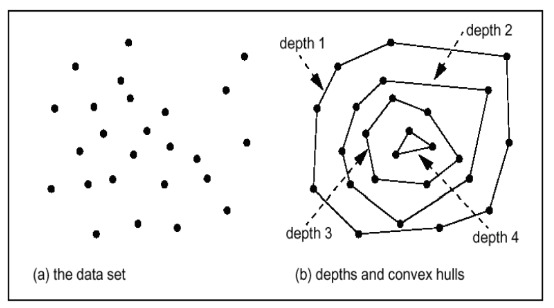
\includegraphics[width=0.5\linewidth]{img/depth_based_od.png}
    \caption{Example of depth-based outlier detection.}
    \label{fig:depth-od}
\end{figure} \\
The points on the convex hull of the full dataset have depth 1. The points in the convex hull of the dataset obtained by removing the points of depth 1 have depth 2, and so on. Once a certain number of convex hulls have been calculated, all points with a depth smaller than some hyperparameter $k$ are reported as outliers. By default it produces a label, but it can be modified so that it returns the depth of each point instead of a 0/1 classification. This algorithm, however, is typically only efficient for two- or three-dimensional spaces. 

Another depth-based algorithm is \textbf{Elliptic Envelope}. It finds the center of the data samples and draws an ellipsoid around it, creating an imaginary elliptical area around the dataset. Instances that fall inside the envelope are considered normal, and anything outside is an outlier. This algorithm works best for data with a Gaussian distribution.

\section{Proximity-based Approaches}

\subsection{Distance-based}

A simple way to define the anomaly score of an instance $x$ is to use its distance to the $k^{th}$ nearest neighbor, $\textit{dist}(x,k)$. If an instance has a lot of close points (so it belongs to the group of normal data), this distance will be small, otherwise the point will be far away from the rest and have a very high distance compared to the rest. Outlier detection algorithms which use $k$-NN distances to score data follow two approaches: either they have a simple \textbf{nested-loop} structure, where a sequential scan computes the $k$-NNs of each instance, or they are \textbf{partition-based}, i.e., they first partition data into micro clusters, and information is aggregated for each partition. This way, micro clusters that cannot qualify when searching for the $k$-NNs of a point can be pruned.

Another common algorithm uses two parameters, a radius $\varepsilon$ and a percentage $\pi$, such that a point $p$ is considered an outlier if at most $\pi$ percent of all other points have a distance to $p$ less than $\varepsilon$ ($p$ is close to very few points). Formally, the set of outliers is computed as:
\begin{equation*}
    \textit{OutlierSet}(\varepsilon, \pi) = \left\{ p | \dfrac{\#\{q \in D | \textit{dist}(p,q) < \epsilon}{\# D} \leq \pi \right\}
\end{equation*}

Finally, outliers can be identified using the \textbf{in-degree number}. Given a dataset, the $k$-NN graph is constructed: each vertex is a data point, and each directed edge between two vertices $p$ and $q$ means that $q$ is one of $p$'s k-nearest neighbors. The in-degree of a point is calculated as the number of reverse $k$-NNs (R$k$-NN), i.e., the number of points who have it as a neighbor. If a point has an in-degree lower than some user-defined threshold, it is declared an outlier. This algorithm outputs an outlier label.

\paragraph{Pros} Distance-based approaches are very simple to implement. They do not require any training, since they're model-free.

\paragraph{Cons} Since the outcome depends on distances, they tend to be slow, and they're not as accurate in high-dimensional spaces. Also, they're sensitive to the chosen hyperparameters and to variations in density.

\subsection{Density-based}

The density around an instance can be defined as $n/V(d)$, where $n$ is the number of instances within a given distance, and $V(d)$ is the volume of the neighborhood. Since $V(d)$ is constant for a given $d$, the density is often only represented using $n$ after fixing a value of $d$. Outliers can be defined as points that are in regions of low density, and their anomaly score as the inverse of the density around them (or the inverse of distance to the $k^{th}$ distance, or the inverse of the average distance to $k$ neighbors). However, if the dataset has regions of different density, this approach can present problems (as seen when discussing DBSCAN).

To fix this problem, the \textbf{average relative density} can be used instead. Given a point $x$ and a number of neighbors $k$, it is calculated as:
\begin{equation*}
    \textit{avg. relative density}(x,k) = \dfrac{\textit{density}(x,k)}{\sum_{y \in N(x,k) \textit{density}(y,k)/|N(x,k)|}}
\end{equation*}
where $N(x,k)$ is the $k$-nearest neighbor of $x$. This way, the density around a point depends on that of its nearest neighbors. If the dataset has areas with differing densities, points in lower density areas will not be classified as outliers. If a point is so faraway that its normal density is high, this relative density will also be high. However, if a point is an outlier only for a very dense cluster, it may not be identified (such as the situation in the figure below).
\begin{figure}[ht]
    \centering
    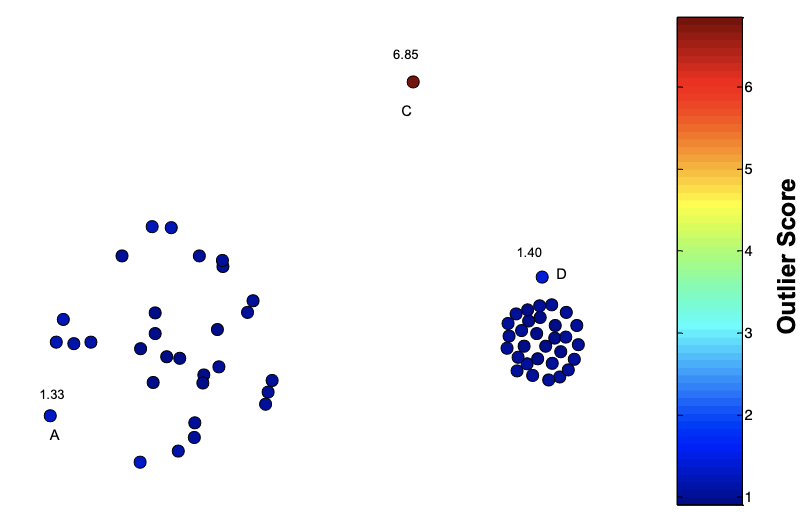
\includegraphics[width=0.5\linewidth]{img/relative_density.png}
    \caption{An example in which average relative density fails. Notice how point $D$ is an outlier for the denser cluster, but it is treated as a normal point.}
    \label{fig:relative-dist}
\end{figure}

\subsubsection{Local Outlier Factor (LOF)}

An alternative is using the \textbf{Local Outlier Factor} (\textbf{LOF}). First, for each pair of points $p$ and $o$ in the dataset, their \textbf{reachability distance}is calculated, identical to that used in OPTICS:
\begin{equation*}
    \textit{reachability-dist}_k(p,o) = \max \{\textit{k-dist}(o), \textit{dist}(p,o)\}
\end{equation*}
then, each point is associated with its \textbf{local reachability distance}:
\begin{equation*}
    \textit{LRD}_k(p) = 1 / \dfrac{\sum_{o \in \textit{N}_k(p)} \textit{reach.-dist}_k(p,o)}{k}
\end{equation*}
Finally, the LOF is calculated as:
\begin{equation*}
    \textit{LOF}_{\textit{k}}(p) = \dfrac{\sum_{o \in N_{k(p)}} \textit{LRD}_{k(o)} / \textit{LRD}_{k(p)} }{k}
\end{equation*}
If a point's LOF is close to 1, then the point is inside a cluster, and if it is much greater than 1, it is an outlier. The result is influenced by the chosen $k$, but an increase in $k$ does not necessarily mean an increase in LOF.

\subsubsection{Connectivity-based Outlier Factor (COF)}

Sometimes, in regions of low density, LOF may fail to detect outliers, unless we use a small $k$. However, using a too small $k$ may include outliers as normal points. A solution is using the \textbf{Connectivity-based Outlier Factor}. It uses \textbf{chaining distance} to calculate a point's nearest neighbor. The average chaining distance is calculated as:
\begin{equation*}
    \textit{ac-dist}_{N_{k(p)}}(p) = \sum_{i=1}^{r-1} \dfrac{2(r-i)}{r(r-1)} CDS_i
\end{equation*}
where $r$ is the number of neighbors in $p$'s $k$-neighborhood, and $CDS_i$ is the cost description sequence of removing the $i^{th}$ neighbor. The chaining distance for a point can be seen as the minimum of the total sum of the distances linking all neighbors. In practice, it is calculated with a graph-like structure. \\
The COF is then calculated as:
\begin{equation*}
    \textit{COF}_k(p) = \dfrac{|N_k(p)| \textit{ac-dist}_{N_{k(p)}}}{\sum_{o \in N_{k(p)}} \textit{ac-dist}_{N_{k(o)}}(o)}
\end{equation*}

\subsubsection{INFLuenced Outlierness (INFLO)}

Another issue that the previous methods fail to address is if clusters of different densities are not well separated.
\begin{figure}[ht]
    \centering
    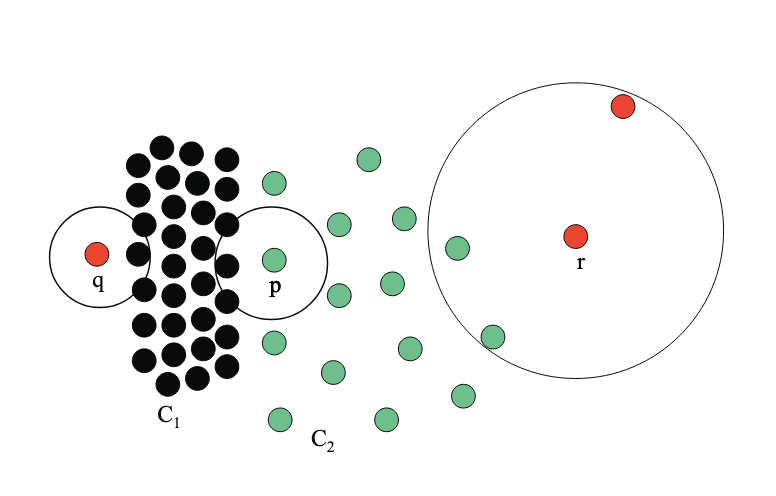
\includegraphics[width=0.5\linewidth]{img/inflo.png}
    \caption{In this example, points $q$ and $r$ have a lower LOF compared to $p$, despite it not being an outlier for the sparse cluster on the right.}
    \label{fig:inflo}
\end{figure}
The idea behind INFLO is to take symmetric neighborhood relationships into account. In other words, it considers both nearest neighbors as well as the reverse nearest neighbors (that is, the points having $p$ as a neighbor), defining the \textbf{influence space} of a point $p$ (indicated with $kIS(p)$).

Density is simply calculated as the inverse of the $k$-distance of a point. The INFLO is then calculated as:\begin{equation*}
    \textit{INFLO}_k(p) = \dfrac{\sum_{o \in kIS(p)} \dfrac{\textit{dens}(o)}{\# kIS(p)}}{dens(p)}
\end{equation*}
Similarly to LOF, if it is close to 1 the point is in a cluster, if instead it is much greater than 1, the point is an outlier.

\paragraph{Pros} Density-based approaches are, like distance based ones, very simple to implement.

\paragraph{Cons} They're computationally expensive since there is a need to find the distance between all points in the dataset, and densities are less meaningful as the dimensionality of the data increases. They are sensitive to the chosen hyperparameters.

\section{Clustering-based Approaches}

Cluster-based outliers are points that do not fit strongly into any cluster. For prototype-based clusters, it means they are far away from it; for density-based clusters, it means the object has a too low density around it; for graph-based clusters, it means the point in not well connected.

Some clustering algorithms are already capable of separating points belonging to clusters from outliers (DBSCAN, OPTICS). An idea would be to simply execute those algorithms feeding the dataset and choosing the appropriate hyperparameters, and analyze the set of ``noise'' points returned by them. However, these are first and foremost clustering algorithms: they are not optimized to find outliers and sets of abnormal data objects may be recognized as a cluster instead of outliers.

Just as we have seen for density-based outliers, we can use \textbf{Cluster-Based Local Outlier Factor} (\textbf{CBLOF}). To calculate it, first a clustering algorithm is used to find clusters in the dataset. Then, each cluster is classified as either a \textbf{small cluster} (\textbf{SC}), or \textbf{large cluster} (\textbf{LC}), using two parameters, $\alpha$ and $\beta$. Specifically, given the clustering $C = \{C_1, C_2, \dots, C_k \}$ such that $|C_1| \geq |C_2| \geq \dots \geq |C_k|$, a boundary $b$ is found if one of the following inequalities hold:
\begin{gather*}
    |C_1| + |C_2| + \dots + |C_b| \geq |D|*\alpha \\
    |C_b|/|C_{b+1} \geq \beta
\end{gather*}
This means that all clusters up until the $b^{th}$ contain $\alpha \%$ of the data points (first formula), or that the smallest of the large clusters must be at least $\beta$ times larger than the larger of the small clusters (second formula). 

The CBLOF is calculated depending on the size of the cluster the point belongs to, as well as the distance to the nearest large cluster. If the point is in a LC, the outlier score is the product between the size of the cluster and the distance with the cluster center. If it is in a SC, the score is the product between the size of the cluster and the distance to the center of the closest LC.
\begin{equation*}
    CBLOF(p) = \begin{cases}
        |C_i|*\min(d(p, C_j)), p \in C_i \land C_j \in LC & \text{if $C_i \in SC$} \\
        |C_i|*d(p, C_i) & \text{if $C_i \in LC$}
    \end{cases}
\end{equation*}

\paragraph{Pros} Cluster-based approaches are simple to implement and a variety of different algorithms exist.

\paragraph{Cons} A main issue is that the presence of outliers itself will distort the clustering. Also, it may be difficult choosing the appropriate hyperparameters and number of clusters when we don't have any knowledge about the structure of the data.

\section{High-dimensional Approaches}

All the approaches seen until now have one big problem in common: they are affected by the curse of dimensionality, and so they don't work well in high-dimensional spaces. An alternative to considering distances is instead considering angles, with \textbf{angle-based outlier detection}. The idea is to compare the angles between pairs of distance vectors that start from the same point. If a point is inside a cluster of data, most angles forming between distance vectors connecting that point and all other points will differ widely. For outliers, instead, all those angles will be similar to each other.
\begin{figure}[ht]
    \centering
    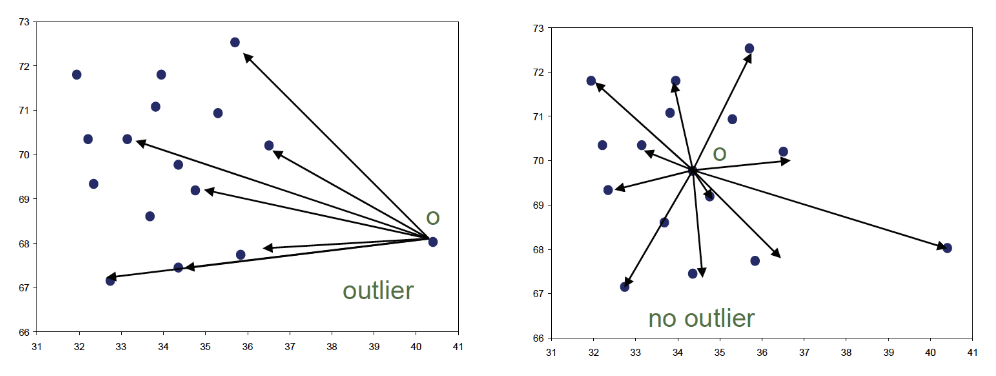
\includegraphics[width=0.7\linewidth]{img/angle_based_od.png}
    \caption{Intuition behind angle-based outlier detection.}
    \label{fig:angle-based}
\end{figure}
For each point $p$, the angle between any two other instances is calculated. The spectrum of all these angles is computed, and depending on its broadness, a score can be assigned to $p$: a small spectrum assigns an high outlier score, a large spectrum assign a small outlier score. Specifically, the \textbf{angle-based outlier degree} (\textbf{ABOD}) is assigned to $p$, calculated as the variance of the angle spectrum weighted by the corresponding distances:
\begin{equation*}
    \textit{ABOD}(p) = \underset{x,y \in D}{\mathrm{Var}} \left ( \dfrac{< \vec{xp}, \vec{yp} >}{\|\vec{xp}\|^2 \cdot \|\vec{yp}\|^2}  \right )
\end{equation*}
Note that the lower the ABOD, the more likely a point is to be an outlier.

The naive algorithm that calculates these degrees has a cost of $O(n^3)$, but it can be approximated by using random sampling to mine the top-$n$ outliers; ABOD is calculated only on the pairs of points in the sample, finding a lower bound of the real ABOD, and filtering out points that have a high ABOD lower bound. The real ABOD is only calculated for a small number of points.

A second approach is called \textbf{grid-based subspace outlier detection}. The data space of $k$ dimensions is partitioned into an equi-depth grid of $\Phi$ cells. The \textbf{sparsity coefficient} of a grid cell $C$ is:
\begin{equation*}
    S(C) = \dfrac{\textit{count}(C) - n (1/ \Phi)^k}{\sqrt{n(1/\Phi)^k (1-(1/\Phi)^k)}}
\end{equation*}
where $\textit{count}(C)$ is the number of data objects in $C$. If $S(C) < 0$, then $\textit{count}(C)$ is lower than expected: all points in those cells are labeled as outliers. This algorithm has a cost of $O(\Phi k)$.

This is a very coarse model: all the points within a cell with low sparsity are automatically outliers, without doing any further analysis on those points, so the quality of the result depends on the grid resolution and position. 

\section{Ensemble-based Approaches}

Ensemble-based means that a group of methods is used on the same dataset, and the final result will be a combination of their singular outcomes. For outlier detection, \textbf{feature bagging} (\textbf{FeaBag}) is used: a set of different outlier detection methods is selected, and each of them is applied on a random set of features selected from the original feature space. Each method will identify different outliers, assigning them outlier scores. The average of those scores is then returned for each point.

An extension of histogram-based outlier score is \textbf{lighteight on-line detector of anomalies} \textbf{(LODA)}. It is especially useful in real-time scenarios where a big amount of records must be processed. LODA approximates the joint probability using a collection of one-dimensional histograms, each constructed on an input space projected onto a randomly generated vector. Even thoug one-dimensional histograms are weak outlier detection methods by themselves, their collection yields good results.

\section{Model-based Approaches}

\textbf{Isolation forests} are a model specialized for outlier detection. First, a set of trees is initialized. Then, each tree receives a different sample of the data. The construction of the tree is done by repeating the following steps until the entire structure is complete, isolating each point in a leaf:
\begin{enumerate}
    \item Pick a random dimension;
    \item Pick a random value on that dimension;
    \item Draw a separating hyperplane at that value, and split the data in the two sides the hyperplanes separates them.
\end{enumerate}
Outliers will tend to be separated in few steps (so the leaves containing them will have low depth), while normal points will be separated after a long time (so they will be found in the deeper leaves). \\
Given a dataset of size $n$, the outlier score of a point $x$ is:
\begin{equation*}
    s(x,n) = 2^{\dfrac{-\mathrm{E}[h(x)]}{c(n)}}
\end{equation*}
where $h(x)$ represents the path length from the root to $x$, and $c(n)$ is the average $h(x)$ given $m$, calculated as:
\begin{equation*}
    c(m) = \begin{cases}
        1 & n = 2 \\
        2 * H(n-1) - \dfrac{2(n-1)}{n} & n > 2 \\
        0 & \text{else}
    \end{cases}
\end{equation*}
$H(i) = \ln(i) + \gamma, \gamma \approx 0.57$ is the $i^{th}$ \hyperlink{https://en.wikipedia.org/wiki/Harmonic_number}{harmonic number}.
\begin{figure}[ht]
    \centering
    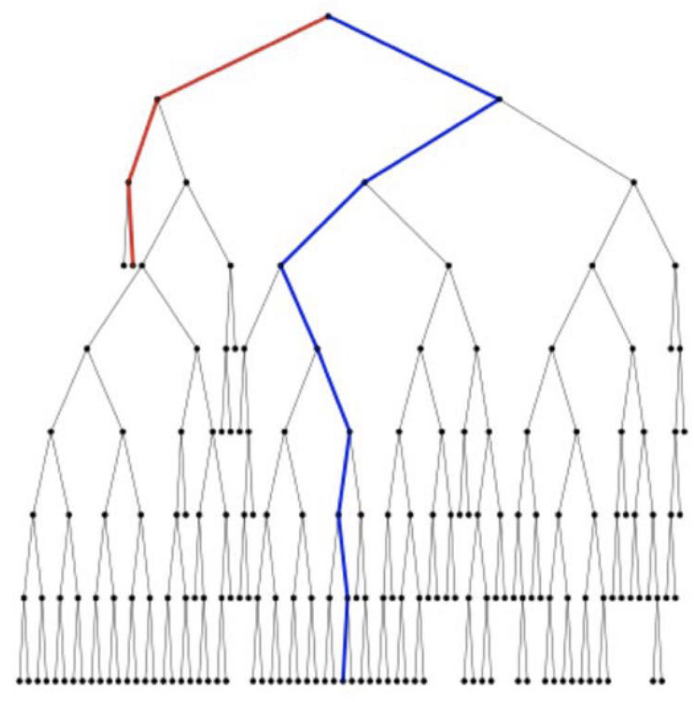
\includegraphics[width=0.35\linewidth]{img/isolation_tree.png}
    \caption{An example of tree: in red the path from the root to an anomaly, in blue the path to a normal point.}
    \label{fig:isolation-tree}
\end{figure}
Isolation forests are computationally efficient, paralellizable, and can handle high dimensional data. However, inconsistent scoring can be observed since the space is always split across one dimension at a time. The \textbf{extended isolation forest} model solves this problem: instead of choosing a dimension, each tree randomly selects both a normal vector and an intercept describing an angled hyperplane.
\clearpage
\begin{figure}[ht]
    \centering
    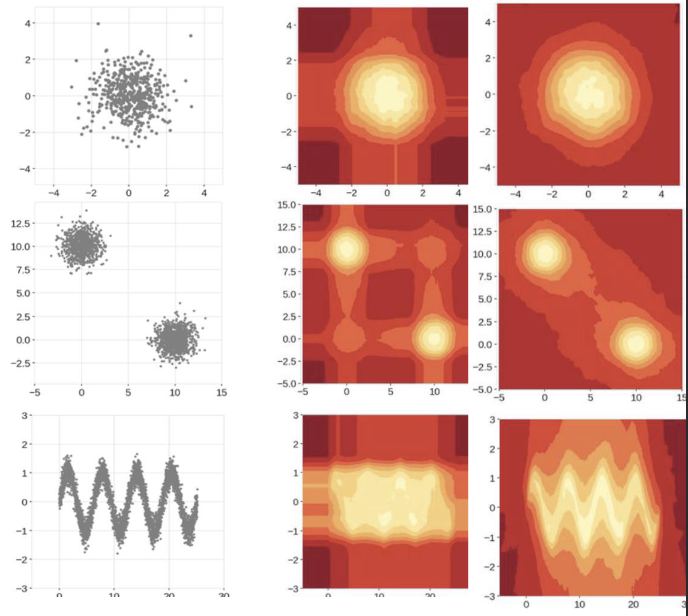
\includegraphics[width=0.5\linewidth]{img/isolation_forests.png}
    \caption{Isolation forests and Extended isolation forests, compared.}
    \label{fig:isolation-forests}
\end{figure}
